\chapter{Interface or Type Relationships}\doublelabel{interface-or-type-relationships}

A class or component, e.g. denoted A, can in some cases be used at a
location designed for another class or component, e.g. denoted B. In
Modelica this is the case for replaceable classes (see \ref{redeclaration}) and
for inner/outer elements (see \ref{instance-hierarchy-name-lookup-of-inner-declarations}). 
Replaceable classes are the
primary mechanism to create very flexible models. In this chapter, the
precise rules are defined when A can be used at a location designed for
B. The restrictions are defined in terms of compatibility rules
(\ref{interface-compatibility-or-subtyping} and \ref{plug-compatibility-or-restricted-subtyping}) between ''interfaces'' (\ref{the-concepts-of-type-interface-and-subtype}); this can
also be viewed as sub-typing (\ref{the-concepts-of-type-interface-and-subtype}).

In this chapter, two kinds of terminology is used for identical concepts
to get better understanding {[}\emph{e.g. by both engineers and computer
scientists}{]}. A short summary of the terms is given in the following
table. The details are defined in the rest of this chapter.

\begin{longtable}{|p{4cm}|p{8cm}|} 
\hline \endhead
\textbf{term} & \textbf{description}\\ \hline
type or interface
& The ``essential'' part of the public declaration sections of a class
that is needed to decide whether A can be used instead of B
{[}\emph{E.g. a declaration ``}Real x\emph{'' is part of the type, also
called interface, but ``}import A\emph{'' is not}{]}.
\\ \hline
\begin{tabular}{@{}p{4cm}@{}}
class type or\\
inheritance interface
\end{tabular}
& 
The ``essential'' part of the public \emph{and protected} declaration
sections of a class that is needed to decide whether A can be used
instead of B. The class type , also called inheritance interface, is
needed when inheritance takes place, since then the protected
declarations have to be taken into account.\\ \hline
\begin{tabular}{@{}p{4cm}@{}}
subtype or\\
compatible interface
\end{tabular} & 
A is a subtype of B, or equivalently, the interface of A is compatible
to the interface of B, if the ``essential'' part of the public
declaration sections of B is also available in A {[}\emph{E.g., if B has
a declaration ``}Real x\emph{'', this declaration must also be present
in A. If A has a declaration ``Real y'', this declaration must not be
present in B}{]}.\\ \hline
\begin{tabular}{@{}p{4cm}@{}}
restricted subtype or
plug compatible interface
\end{tabular} & 
A is a restricted subtype of B, or equivalently, the interface of A is
plug compatible to the interface of B, if A is a subtype of B and if
connector components in A that are not in B, are default connectable.
{[}\emph{E.g. it is not allowed that these connectors have variables
with the ``input'' prefix, because then they must be connected.}{]} A
model or block A cannot be used instead of B, if the particular
situation does not allow to make a connection to these additional
connectors. In such a case the stricter ``plug compatible'' is required
for a redeclaration.\\ \hline
\begin{tabular}{@{}p{4cm}@{}}
function subtype or\\
function compatible interface
\end{tabular} & 
A is a function subtype of B, or equivalently, the interface of A is
function compatible to the interface of B, if A is a subtype of B and if
the additional arguments of function A that are not in function B are
defined in such a way, that A can be called at places where B is called.
{[}\emph{E.g. an additional argument must have a default
value.}{]}\\ \hline
\end{longtable}

\section{The Concepts of Type, Interface and Subtype}\doublelabel{the-concepts-of-type-interface-and-subtype}

A \emph{type} can conceptually be viewed as a \emph{set of values}. When
we say that the variable x has the type Real, we mean that the value of
x belongs to the set of values represented by the type Real i.e.,
roughly the set of floating point numbers representable by Real, for the
moment ignoring the fact that Real is also viewed as a class with
certain attributes. Analogously, the variable b having Boolean type
means that the value of b belongs to the set of values \{false, true\}.
The built-in types Real, Integer, String, Boolean are considered to be
distinct types.

The \emph{subtype} relation between types is analogous to the subset
relation between sets. A type A1 being a subtype of type A means that
the set of values corresponding to type A1 is a subset of the set of
values corresponding to type A.

The type Integer is not a subtype of Real in Modelica even though the
set of primitive integer values is a subset of the primitive real values
since there are some attributes of Real that are not part of Integer
(\ref{predefined-types-and-classes}).

The concept of \emph{interface} as defined in \ref{interface-or-type} and used in
this document is equivalent to the notion of type based on sets in the
following sense:

An element is characterized by its interface defined by some attributes
(\ref{interface-or-type}). The \emph{type} of the element is the set of values
having the same interface, i.e. the same attributes.

A \emph{subtype} A1 in relation to another type A, means that the
elements of the set corresponding to A1 is a subset of the set
corresponding to A, characterized by the elements of that subset having
additional properties.

{[}\emph{Example}:

\emph{A record} R: record R Boolean b; Real x; end R;

\emph{Another record called} R2: R2 Boolean b; Real x; Real y; end R2;

\emph{An instance} r: R r;

\emph{An instance} r2: R2 r2;

\emph{The type} R \emph{of} r \emph{can be viewed as the set of all
record values having the attributes defined by the interface of}
R\emph{, e.g. the infinite set} \{R(b=false,x=1.2), R(b=false, x=3.4),
R(b=true, x=1.2), R(b=true, x=1.2, y=2), R(b=true, x=1.2,
a=2),...)\emph{. The statement that} r \emph{has the type (or
interface)} R \emph{means that the value of} r \emph{belongs to this
infinite set}.

\emph{The type} R2 \emph{is a subtype of} R \emph{since its instances
fulfill the additional property of having the component} Real y;
\emph{in all its values.}{]}

\begin{figure}
\caption{The type R can be defined as the set of
record values containing x and b. The subtype R2 is the subset of values
that all contain x, b, and y.}
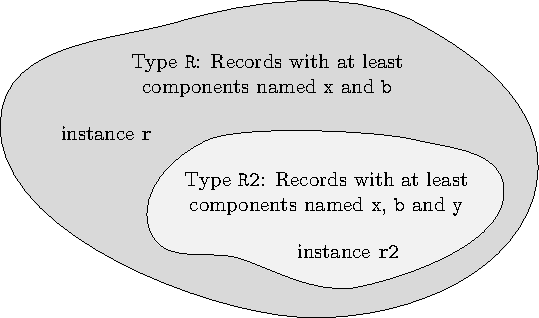
\includegraphics{media/subtype.pdf}
\end{figure}
{]}

\section{Interface or Type}\doublelabel{interface-or-type}

Based on a flattened class or component we can construct an interface
for that flattened class or component. The interface or type
{[}\emph{the terms interface and type are equivalent and can be used
interchangeably}{]} is defined as the following information about the
flattened element itself:

\begin{itemize}
\item
  Whether it is replaceable or not.
\item
  Whether the class itself or the class of the component is transitively
  non-replaceable (\ref{transitively-non-replaceable}), and if not, the reference to the
  replaceable class it refers to.
\item
  Whether it is a component or a class.
\item
  Additional information about the element:

  \begin{itemize}
  \item
    The flow- or stream-prefix.
  \item
    Declared variability (constant, parameter, discrete).
  \item
    The prefixes input and output.
  \item
    The prefixes inner and/or outer.
  \item
    Whether the declaration is final, and in that case its semantics
    contents.
  \item
    Array sizes (if any).
  \item
    Condition of conditional components (if any).
  \item
    Which kind of specialized class.
  \item
    For an enumeration type or component of enumeration type the names
    of the enumeration literals in order.
  \item
    Whether it is a built-in type and the built-in type (RealType,
    IntegerType, StringType or BooleanType).
  \end{itemize}
\item
  Only for an operator record class and classes derived from
  ExternalObject: the full name of the operator record base-class (i.e.
  the one containing the operations), or the derived class. See 
  \ref{overloaded-operators} and \ref{external-objects}.\\
  The following item does not apply for an operator record class or
  class derived from ExternalObject, since the type is already uniquely
  defined by the full name.
\item
  For each named public element of the class or component (including
  both local and inherited named elements) a tuple comprised of:

  \begin{itemize}
  \item
    Name of the element.
  \item
    Interface or type of the element. \emph{This might have been
    modified by modifiers and is thus not necessarily identical to the
    interface of the original declaration}.
  \end{itemize}
\end{itemize}

The corresponding \emph{constraining} interface is constructed based on
the \emph{constraining} type (\ref{constraining-type}) of the declaration (if
replaceable -- otherwise same as actual type) and with the
\emph{constraining} interface for the named elements.

In a class all references to elements of that class should be limited to
their constraining interface \emph{(i.e. only public elements and if the
declaration is replaceable limited to the constraining interface)}.

{[}\emph{The public interface does not contain all of the information
about the class or component. When using a class as a base-class we also
need protected elements, and for internal type-checking we need e.g.
import-elements. However, the information is sufficient for checking
compatibility and for using the class to flatten components.}{]}

\subsection{Transitively non-Replaceable}\doublelabel{transitively-non-replaceable}

{[}\emph{In several cases it is important that no new elements can be
added to the interface of a class, especially considering short class
definitions. Such classes are defined as transitively
non-replaceable.}{]}

A class reference is transitively non-replaceable iff (i.e. ``if and
only if'') all parts of the name satisfy the following:

\begin{itemize}
\item
  If the class definition is long it is transitively non-replaceable if
  not declared replaceable.
\item
  If the class definition is short (i.e. `class A=P.B') it is
  transitively non-replaceable if it is non-replaceable and equal to
  class reference (``P.B'') that is transitively non-replaceable.
\end{itemize}

{[}\emph{According to \ref{restrictions-on-base-classes-and-constraining-types-to-be-transitively-non-replaceable}, for a hierarchical name all
parts of the name must be transitively non-replaceable, i.e. in
``extends A.B.C'' this implies that A.B.C must be transitively
non-replaceable, as well as A and A.B, with the exception of the ``class
extends redeclaration mechanism'' see \ref{the-class-extends-redeclaration-mechanism}}{]}

\subsection{Inheritance Interface or Class Type}\doublelabel{inheritance-interface-or-class-type}

For inheritance the interface also must include protected elements; this
is the only change compared to above.

Based on a flattened class we can construct an inheritance interface or
class type for that flattened class. The inheritance interface or class
type is defined as the following information about the flattened element
itself:

\begin{itemize}
\item
  Whether it is replaceable or not.
\item
  Whether the class itself or the class of the component is transitively
  non-replaceable (\ref{transitively-non-replaceable}), and if not the reference to
  replaceable class it refers to.
\item
  For each named element of the class (including both local and
  inherited named elements) a tuple comprised of:

  \begin{itemize}
  \item
    Name of the element.
  \item
    Whether the element is component or a class.
  \item
    For elements that are classes: Inheritance interface or class type
    of the element. \emph{This might have been modified by modifiers and
    is thus not necessarily identical to the interface of the original
    declaration}.
  \item
    For elements that are components: interface or type of the element.
    \emph{This might have been modified by modifiers and is thus not
    necessarily identical to the interface of the original declaration}.
  \end{itemize}
\item
  Additional information about the element:

  \begin{itemize}
  \item
    The flow- or stream-prefix.
  \item
    Declared variability (constant, parameter, discrete).
  \item
    The prefixes input and output.
  \item
    The prefixes inner and/or outer.
  \item
    Whether the declaration is final, and in that case its semantics
    contents.
  \item
    Array sizes (if any).
  \item
    Condition of conditional components (if any).
  \item
    Which kind of specialized class.
  \item
    For an enumeration type or component of enumeration type the names
    of the enumeration literals in order.
  \item
    Whether it is a built-in type and the built-in type (RealType,
    IntegerType, StringType or BooleanType).
  \item
    Visibility (public or protected).
  \end{itemize}
\end{itemize}

\section{Interface Compatibility or Subtyping}\doublelabel{interface-compatibility-or-subtyping}

An interface of a class or component A is compatible with an interface
of a class or component B (or the constraining interface of B), or
equivalently that the type of A is a subtype of the type of B, iff
{[}\emph{intuitively all important elements of B must be present in A}
{]}\emph{:}

\begin{itemize}
\item
  A is a class if and only if B is a class (and thus: A is a component
  if and only if B is a component).
\item
  If A has an operator record base-class then B must also have one and
  it must be the same. If A does not have an operator record base-class
  then B may not have one. See \ref{overloaded-operators}.
\item
  If A is derived from ExternalObject, then B must also be derived from
  ExternalObject and have the same full name. If A is not derived from
  ExternalObject then B may not derived from ExternalObject. See 
  \ref{external-objects}.
\item
  If B is not replaceable then A may not be replaceable.
\item
  If B is transitively non-replaceable then A must be transitively
  non-replaceable (\ref{transitively-non-replaceable}). For all elements of the inheritance
  interface of B there must exist a compatible element with the same
  name and visibility in the inheritance interface of A. The interface
  of A may not contain any other elements. {[}\emph{We might even extend
  this to say that A and B should have the same contents, as in the
  additional restrictions below.}{]}
\item
  If B is replaceable then for all elements of the component interface
  of B there must exist a plug-compatible element with the same name in
  the component interface of A.
\item
  If B is neither transitively non-replaceable nor replaceable then A
  must be linked to the same class, and for all elements of the
  component interface of B there must thus exist a plug-compatible
  element with the same name in the component interface of A.
\item
  Additional restrictions on the additional information. These elements
  should either match or have a natural total order:

  \begin{itemize}
  \item
    If B is a non-replaceable long class definition A must also be a
    long class definition.
  \item
    The flow-or stream-prefix should be matched for compatibility.
  \item
    Variability is ordered constant\textless{} parameter\textless{}
    discrete\textless{} (no prefix: continuous-time for Real), and A is
    only compatible with B if the declared variability in A is less than
    or equal the variability in B. \emph{For a redeclaration of an
    element the variability prefix is as default inherited by the
    redeclaration (i.e. no need to repeat `parameter' when redeclaring a
    parameter).}
  \item
    The input and output prefixes must be matched. This ensures that the
    rules regarding inputs/outputs for matching connectors and
    (non-connector inputs) are preserved, as well as the restriction on
    blocks. \emph{For a redeclaration of an element the input or output
    prefix is inherited from the original declaration.}
  \item
    The inner and/or outer prefixes should be matched. \emph{For a
    redeclaration of an element the} inner \emph{and/or} outer
    \emph{prefixes are inherited from the original declaration (since it
    is not possible to have} inner \emph{and/or} outer \emph{as part of
    a redeclare)}.
  \item
    If B is final A must also be final and have the same semantic
    contents.
  \item
    The number of array dimensions in A and B must be matched.
  \item
    Conditional components are only compatible with conditional
    components. The conditions must have equivalent contents (similar as
    array sizes -- except there is no ``:'' for conditional components).
    \emph{For a redeclaration of an element the conditional part is
    inherited from the original.}
  \item
    A function class is only compatible with a function class, a package
    class only compatible with a package class, a connector class only
    with a connector class, a model or block class only compatible with
    a model or block class, and a type or record class only compatible
    with a type or record class.
  \item
    If B is an enumeration type A must also be an enumeration type and
    vice versa. If B is an enumeration type not defined as (:) then A
    must have the same enumeration literals in the same order; if B is
    an enumeration type defined as (:) then there is no restriction on
    the enumeration type A.
  \item
    If B is a built-in type then A must also be of the same built-in
    type and vice versa.
  \end{itemize}
\end{itemize}

Plug-compatibility is a further restriction of compatibility (subtyping)
defined in \ref{plug-compatibility-or-restricted-subtyping}, and further restricted for functions, see
\ref{function-compatibility-or-function-subtyping-for-functions}. For a replaceable declaration or modifier the default class
must be compatible with the constraining class.

For a modifier the following must apply:

\begin{itemize}
\item
  The modified element should exist in the element being modified.
\item
  The modifier should be compatible with the element being modified, and
  in most cases also plug-compatible, \ref{plug-compatibility-or-restricted-subtyping}.
\end{itemize}

{[}\emph{If the original constraining flat class is legal (no references
to unknown elements and no illegal use of class/component), and
modifiers legal as above -- then the resulting flat class will be legal
(no references to unknown elements and no illegal use of class/component
and compatible with original constraining class) and references refer to
similar entities.}{]}

\section{Plug-Compatibility or Restricted Subtyping}\doublelabel{plug-compatibility-or-restricted-subtyping}

{[}\emph{If a sub-component is redeclared, see \ref{redeclaration}, it is
impossible to connect to any new connector. A connector with input
prefix must be connected to, and since one cannot connect across
hierarchies, one should not be allowed to introduce such a connector at
a level where a connection is not possible. Therefore all public
components present in the interface A that are not present in B must be
connected by default.}{]}

Definition 5: Plug-compatibility (= restricted subtyping)

An interface A is plug-compatible with (a restricted subtype of) an
interface B (or the constraining interface of B) iff:

\begin{itemize}
\item
  A is compatible with (subtype of) B.
\item
  All public components present in A but not in B must be
  default-connectable (as defined below).
\end{itemize}

Definition 6: Default connectable

A component of an interface is default-connectable iff:

\begin{itemize}
\item
  All of its components are default connectable.
\item
  A connector component must not be an input. {[}\emph{Otherwise a
  connection to the input will be missing.}{]}
\item
  A connector component must not be of an expandable connector class.
  {[}\emph{The expandable connector does potentially have inputs.}{]}
\item
  A parameter, constant, or non-connector input must either have a
  binding equation or all of its sub-components must have binding
  equations.
\end{itemize}

Based on the above definitions, there are the following restrictions:

\begin{itemize}
\item
  A redeclaration of an inherited top-level component must be
  \emph{compatible} \emph{with} (subtype of) the constraining interface
  of the element being redeclared.
\item
  In all other cases redeclarations must be \emph{plug-compatible} with
  the constraining interface of the element being redeclared.
\end{itemize}

{[}\emph{The reason for the difference is that for an inherited
top-level component it is possible to connect to the additional
connectors, either in this class or in a derived class.}

\emph{Example:}
\begin{lstlisting}[language=modelica]
partial model TwoFlanges
  Modelica.Mechanics.Rotational.Interfaces.Flange_a flange_a;
  Modelica.Mechanics.Rotational.Interfaces.Flange_b flange_b;
end TwoFlanges;

partial model FrictionElement
  extends TwoFlanges;
  ...
end FrictionElement;

model Clutch "compatible - but not plug-compatible with FrictionElement"
  Modelica.Blocks.Interfaces.RealInput pressure;
  extends FrictionElement;
  ...
end Clutch;

model DriveLineBase
  extends TwoFlanges;
  Inertia J1;
  replaceable FrictionElement friction;
equation 
  connect(flange_a, J1.flange_a);
  connect(J1.flange_b, friction.flange_a);
  connect(friction.flange_b, flange_b);
end DriveLineBase;

model DriveLine
  extends DriveLineBase(redeclare Clutch friction);
  Constant const;
equation 
  connect(const.y, frition.pressure);
  // Legal connection to new input connector.
end DriveLine;

model UseDriveLine "illegal model"
  DriveLineBase base(redeclare Clutch friction);
  // Cannot connect to friction.pressure
end UseDriveLine;
\end{lstlisting}

\emph{If a subcomponent is redeclared, it is impossible to connect to
any new connector. Thus any new connectors must work without being
connected, i.e., the default connection of flow-variables. That fails
for inputs (and expandable connectors may contain inputs). For
parameters and non-connector inputs it would be possible to provide
bindings in a derived class, but that would require hierarchical
modifiers and it would be bad modeling practice that a hierarchical
modifier must be used in order to make a model valid. A replaceable
class might be used as the class for a sub-component, therefore
plug-compatibility is required not only for replaceable sub-components,
but also for replaceable classes.}{]}

\section{Function-Compatibility or Function-Subtyping for Functions}\doublelabel{function-compatibility-or-function-subtyping-for-functions}

{[}\emph{Functions may be called with either named or positional
arguments, and thus both the name and order is significant. If a
function is redeclared, see \ref{redeclaration}, any new arguments must
have defaults (and be at the end) in order to preserve the meaning of
existing calls.}{]}

Definition 7: Function-Compatibility or Function-Subtyping for Functions

A function class A is \emph{function-compatible with or a function
subtype of} function class B iff, {[}\emph{The terms function-compatible
and function subtype of are synonyms and used interchangeably}{]}:

\begin{itemize}
\item
  A is compatible to (subtype of) B.
\item
  All public input components of B have correspondingly named public
  input components of A in the same order and preceding any additional
  public input components of A.
\item
  All public output components of B have correspondingly named public
  output components of A in the same order and preceding any additional
  public output components of A.
\item
  A public input component of A must have a binding assignment if the
  corresponding named element has a binding assignment in B.
\item
  A public input component of A not present in B must have a binding
  assignment.
\end{itemize}

Based on the above definition the following restriction holds:

\begin{itemize}
\item
  The interface of a redeclared function must be
  \emph{function-compatible with or a function subtype of} the
  constraining interface of the function being redeclared.
\end{itemize}

{[}\emph{Example: Demonstrating a redeclaration using a
function-compatible function}
\begin{lstlisting}[language=modelica]
function GravityInterface
  input Modelica.SIunits.Position position[3];
  output Modelica.SIunits.Acceleration acceleration[3];
end GravityInterface;

function PointMassGravity
  extends GravityInterface;
  input Modelica.SIunits.Mass m;
algorithm 
  acceleration := -Modelica.Constants.G*m*position/(position*position)^1.5;
end PointMassGravity;

model Body
  model UseDriveLine "illegal model"
    DriveLineBase base(redeclare Clutch friction);
    // Cannot connect to friction.pressure
  end UseDriveLine;
  Modelica.Mechanics.MultiBody.Interface.Frame_a frame_a;
  replaceable function gravity = GravityInterface;
equation 
  frame_a.f = gravity(frame_a.r0);
  // or gravity(position=frame_a.r0);
  frame_a.t = zeros(3);
end Body;

model PlanetSimulation
  function sunGravity = PointMassGravity (m=2e30);
  Body planet1(redeclare function gravity = sunGravity);
  Body planet2(redeclare function gravity = PointMassGravity (m=2e30));
  ...
end PlanetSimulation;
\end{lstlisting}

\emph{Note:} PointMassGravity \emph{is not function-compatible with}
GravityInterface \emph{(no default for} m\emph{), but} sunGravity
\emph{inside} PlanetSimulation \emph{is function-compatible with}
GravityInterface\emph{.}{]}

\section{Type Compatible Expressions}\doublelabel{type-compatible-expressions}

Certain expressions consist of an operator applied to two or more type
compatible sub-expressions (A and B), including binary operators, e.g. A
+ B, if-expressions, e.g. if x then A else B, and array expressions,
e.g. \{A,B\}. The resulting type of the expression in case of two type
compatible subexpressions A and B is defined as follows:

\begin{itemize}
\item
  If A is a record-expression B must also be a record-expression with
  the same named elements. The type compatible expression is a record
  comprised of named elements that are compatible with the corresponding
  named elements of both A and B.
\item
  If A is an array expression then B must also be an array expression,
  and ndims(A)=ndims(B). The type compatible expression is an array
  expression with elements compatible with the elements of both A and B.
  If both size(A) and size(B) are known and size(A)=size(B) then this
  defines the size of the type compatible expression, otherwise the size
  of the expression is not known until the expression is about to be
  evaluated. In case of an if-expression the size of the type compatible
  expression is defined based on the branch selected, and for other
  cases size(A)=size(B) must hold at this point.
\item
  If A is a scalar expression of a simple type B must also be a scalar
  expression of a simple type.
\item
  If A is a Real expression then B must be a Real or Integer expression
  and the type compatible expression is Real.
\item
  If A is an Integer expression then B must be a Real or Integer
  expression. For exponentiation and division the type compatible
  expression is Real (even if both A and B are Integer) see 10.610.6, in
  other cases the type compatible expression is Real or Integer (same as
  B).
\item
  If A is a Boolean expression then B must be a Boolean expression and
  the type compatible expression is Boolean.
\item
  If A is a String expression then B must be a String expression and the
  type compatible expression is String.
\item
  If A is an enumeration expression then B must be an enumeration
  expression and the type compatible expression is enumeration
  expression, and all enumeration expressions must be defined in terms
  of an enumeration type with the same enumeration literals in the same
  order.
\item
  If A has an operator record base-class then B must also have an
  operator record base-class, and it must be the same, and otherwise
  neither A nor B may have an operator record base-class. This is also
  the operator record base-class for the expression e.g. for `if (cond)
  then A else B'.
\item
  If A is derived from ExternalObject then B must also be derived from
  ExternalObject and they must have the same full name; and otherwise
  neither A nor B may be derived from ExternalObject. The common full
  name also defines the type of the expression, e.g. for `if (cond) then
  A else B'.
\end{itemize}
